\documentclass{llncs}
\usepackage{graphics}
\usepackage{amssymb}
\usepackage[dvips]{epsfig}
\usepackage[spanish]{babel}
%\usepackage[latin1]{inputenc}

\def\CC{{C\hspace{-.05em}\raisebox{.4ex}{\tiny\bf ++}}~}
\addtolength{\textfloatsep}{-0.5cm}
\addtolength{\intextsep}{-0.5cm}


%%%%%%%%%%%%%%%% Titulo %%%%%%%%%%%%%%%
\title{SIPESCA-B: a set of real data time series benchmark for traffic prediction}

%%%%%%%%%%%%%%%% autores %%%%%%%%%%%%%%%
\author {
P.A. Castillo et al.
}
\institute{Department of Architecture and Computer Technology. CITIC \\
           University of Granada (Spain) \\
~\\
           e-mail: {\tt pacv@ugr.es}}

\date{} 

\begin{document}
\maketitle

%%%%%%%%%%%%%%%%%%%%%%%%%%%%%%%%%%%%%%%%%%%%%%%%%%%%%%%%%%%%%%
\begin{abstract}

In the field of traffic management                                     % management? Prediction? Traffic what? Rate? modelling? 
no public real-data benchmarks are available to the research
community % that we know of, siempre
for testing their information processing methods and compare their
results with those obtained by other researchers.                       % This implies that... or this is bad because... - JJ
In this work the benchmark SIPESCA-B, a set of time series 
obtained monitoring the traffic at several locations in the 
Andalusian road network, is presented. 
Time series are built using real data from the number of vehicles that
have passed through certain locations along several months.             % not _all_ vehicles - JJ
The datasets are provided in simple formats with widespread use and
are left available in a public repository. 
Our aim for this work is to provide public access and details of this benchmark
as well as preliminary results with various prediction methods to the
research community to serve as comparison of future results in the field of
management and traffic prediction. 

\end{abstract}

%\begin{keywords}
  %Traffic flow forecasting, Bluetooth technology, Prediction, Time Series
  %Benchmarks, Traffic Prediction, Bluetooth, Time Series
%\end{keywords}

%********************************************************************************
\section{Introduction}

There are many fields where standard benchmarks are widely used by researchers, such as Proben1 \cite{Prechelt1994} in the artificial neural networks area, or the functional optimization competition benchmark of IEEE Congress on Evolutionary Computation \cite{CEC2014}.

However, in other areas there is a need for this type of real problems, such as in the area of traffic management.
In this area, due to the type of problems, there is a difficulty in obtaining and using real data.
In some cases due to the lack of data in a suitable format \cite{Flyvbjerg2008}, and in other cases because it is confidential commercial data \cite{Bain2009} obtained, i.e., in highway tolls \cite{Kriger2006}. 
Thus, only certain research works can use that data, which makes impossible to compare results with other researchers.

% Department of Infraestructure and Transport. Australian Government. Review the Traffic Forecasting Performance Toll Roads. http://www.infrastructure.gov.au/infrastructure/public_consultations/files/attach_a_bitre_literature_review.pdf
%
% Kriger2006
% toll data  /  data required for traffic modelling may include, among other things, traffic counts, network characteristics and generalised travel costs. These data are sometime lacking or subject to sampling/processing errors
%
%Flyvbjerg2008
% Inappropriate models, poor quality and/or lack of data, and inadequate modelling assumptions are often cited in the literature as the main sources of forecasting errors.
%
% Bain2009
%http://ibtta.org/sites/default/files/Error%20and%20optimism%20in%20traffic%20predictions.pdf
% absence of comparative data
% available toll road data 
% The author had access to commercial-in-confidence documentation [...] compiled a database of predicted and actual traffic usage for over 100 international, privately financed toll road projects
% 
% \cite{Morzy2007}
% Synthetic datasets were generated using Network-based Generator of Moving Objects by T.Brinkhoff \cite{Brinkhoff2002}. 
%
% \cite{PLAISANT2008}
% �facilitate the comparison of different techniques and encourage researchers to work on challenging problems�

That is why many researchers present their work using traffic
simulators \cite{Morzy2007} or artificial benchmarks to obtain data to
which applying data mining or prediction algorithms. % The existence
                                % of benchmarks contradicts what you
                                % said above - JJ
%
% Linear Road Benchmark simulates a variable tolling system [6]
% The system uses the MIT Trac Simulator to generate moving vehicles
%
% The DynaMark Benchmark simulates the movement of mobile users  who update their location with an average periodicity. [14]
%
% COST Benchmark  simulated objects with periodically updated 2-D locations.   [12]
%
% The BerlinMOD benchmark, like LRB, simulates spatio-temporal data of moving vehicles on a road network [9]. 
%
% HE GSMARK BENCHMARK: The resulting data consists of a real road network with simulated moving vehicles \cite{Shen2011}
%
% \cite{Gidofalvi2010}
% data set contains the GPS readings of 1500 taxis and 400 trucks travelling on the streets of Stockholm
%
Among these synthetic benchmarks we can mention:
\begin{itemize}
  \item  \emph{Linear Road Benchmark} uses the \emph{MIT Trac Simulator} to simulate the movement of vehicles on a toll \cite{Arasu2004}.
  \item  \emph{DynaMark Benchmark} simulates the movement of users, updating its position with a certain frequency \cite{Myllymaki2003}.
  \item  \emph{COST Benchmark} simulates moving objects and periodically updates its 2D position \cite{Jensen2006}.
  \item  \emph{BerlinMOD Benchmark} simulates spatio-temporal data from vehicle movements on a real road network \cite{Duntgen2009}.
  \item  \emph{GSMARK Benchmark} generates data from a real road on which simulating the vehicle movements \cite{Shen2011}.
  \item  \emph{Transport and Logistics Division of the Department of Urban Planning and Environment} public benchmark, consisting of real data from the GPS position of 1500 taxis and 400 trucks moving through the streets of Stockholm \cite{Gidofalvi2010}.
\end{itemize}


Thus there is a need for, not only standard benchmarks based on real traffic data, but also rules or conventions about how to use them to evaluate different prediction methods in the traffic management field.
One way to face this problem is to encourage researchers to either use standard benchmarks or publish not only the results but also the problem data along its detailed description.

As stated, it is not enough using a set of problems and rules; researchers should take into account that the results obtained using these problems must be comparable and reproducible.
In order to achieve this, some benchmark results are necessary as a basis for comparisons.

Having the real data based benchmark, application rules, documentation and some results for the sake of comparison, facilitates the researchers' work, ensuring reproducibility and comparability of results \cite{PLAISANT2008}.

In this sense, SIPESCA-B is intended as a first step towards a standard benchmark for the traffic management field. It consist of several time series obtained from real data from passing vehicles through several geographical points of Andalusian roads.
Making it publicly available facilitates the access to researchers to real mobility data, using simple and widespread formats.

In addition, following the recommendations of Prechelt \cite{Prechelt1994}, a set of rules are proposed to carry out the implementation and use of prediction methods to face these problems.

Finally, using real data problems versus artificial or synthetic data problems makes research and its results are relevant in at least one field \cite{Prechelt1994,PLAISANT2008}.


The rest of this paper is organized as follows:
In Section \ref{sec:timeseries}, the research project within this work has been developed is presented. This section details how the time series data has been obtained.
Section \ref{sec:medidasdeerror} proposes several standar measures of error to be used when carrying out the time series predictions, so that the obtained results are comparable with those presented by other authors.
Then, a brief state of the art on methods for predicting time series is presented (Section \ref{sec:ForecastTools}).
In Section \ref{sec:Experiments}, a series of experimental results is presented on several time series, using several prediction methods and the proposed measures of error.
Finally, Section \ref{sec:Conclusions} presents a brief conclusions, followed by future works.


%********************************************************************************
\section{Time series data collection}
\label{sec:timeseries}

Below, the research project in which data from passing vehicles through several roads was obtained, is described. 
Then, the general principles and objectives of the proposed benchmark, named SIPESCA-B, are discussed. Finally, the time series that were used in the experiments presented in Section \ref{sec:Experiments} are described.

\subsection{Data collection. The SIPESCA project}

This work is part of the project \emph{''Sistema de Informaci�n y Predicci�n de bajo coste y aut�nomo para conocer el Estado de las Carreteras en tiempo real mediante dispositivos distribuidos'' (SIPESCA)} \cite{papersipesca1,papersipesca2}.
The main objective of this project was building a low-cost, rapid deployment and high reliability system to provide real-time information about the traffic status and flows that occur in a certain area, allowing to optimally manage motion decisions not only by the institutions and traffic agencies, but also by citizens (i.e. through mobile alerts or through web).

SIPESCA monitoring devices have collected a large amount of data corresponding to passing BT/Wifi devices by various routes of different types (highways, roads and streets in Granada and several towns in the metropolitan area of Seville, Spain).
Taking and analyzing collected data, several time series of passing vehicles have been built. 
Using these time series, the traffic flow on those monitored roads can be predicted.

Data acquisition is based on the detection of Bluetooth (BT) and Wifi devices, which provides a description of the traffic conditions in real time as well as a set of reliable data to carry out traffic prediction using several time series forecasting techniques.
Both BT devices embedded in some kind of vehicle and personal devices with BT or WiFi enabled are detected and accounted.

The system collects the MAC address (\emph{media access control} or physical address, is a 48-bit identifier that uniquely corresponds to a card or network device) of the device BT card as well as the exact time at which it has been detected. 
The MAC is an unique identifier for each device, allowing us to identify passing vehicles. Additionally, analyzing the MAC allows us to determine the manufacturer, model, and even distinguish what type of device it is and its features (i.e. handsfree, PC, mobile phone, etc), as detailed in \cite{IEEEBT} and \cite{WikipediaOUI}.
Data is encrypted and stored allowing to identify just the device, but not the user, so that user privacy is guaranteed.
Proposed acquisition method allows identifying a device in several city locations, which can give an idea of how that device has been moving.

Specifically, the Intelify\footnote{http://www.intelify.net} \cite{Ariza2011} device was used for data acquisition, as it offers a suitable solution to capture BT/Wifi devices. % (it exhibits a 8.5 \% error in data collection). 
Intelify is an autonomous unit that scan the environment and sends the information to a central server using a 3G\footnote{http://en.wikipedia.org/wiki/3G} connection for further processing and interpretation.

Obtained information is organized into an entity called ''pass''. This refers to a device detected on a node at a given start time and up to an specific end time. Thus, the data node, device MAC, start time and end time categorize a step.

Finally, SIPESCA project aim is obtaining information about traffic flows that occur in an area, allowing official organisms and individual road users to optimally manage their motion decisions.


\subsection{SIPESCA-B benchmark}

Publishing the SIPESCA-B benchmark seeks to offer a set of time series, obtained from real data, to practitioners in the field of management and traffic prediction.

Data sets are provided in plain text, using simple and widespread formats (CSV, JSON, ARFF and XML) and are left available in the public code repository {\tt https://github.com/Sipesca/Datasets}
under the Open Database License \footnote{http://opendatacommons.org/licenses/odbl} that allows researchers to copy and distribute data, to create derivative works, and to transform data, if the same license is maintained.

Along with the data sets and the basic rules to use them, a set of predictions obtained using several time series prediction methods are presented. Thus, practitioners can use those predictions as a basis for comparisons.

By using this benchmark, the reproducibility of future experiments can be improved, so that, other researchers can replicate experiments. This is an important point, as the reproducibility is a bedrock requirement of modern science, in order to check the experiments validity.

Furthermore, in many papers authors just cite well-known problems in a diffuse way, such as ''the Glass Proben1 has been used'' \cite{Prechelt1994}.
Those references are confusing, as there may be several versions of the problem, even between different papers authored by the same authors.
In this sense, SIPESCA-B aims to facilitate both the use of well-documented problems, and the comparability of obtained results using different methods. As the problem data is the same, authors just have to specify the time series used and to detail the prediction method and parameters chosen.


\subsection{Time series publication in a public repository}

As stated above, the benchmark is left available in a public repository\footnote{https://github.com/Sipesca/Datasets}, offering the time series in 4 different file formats: CSV, JSON, XML and ARFF.
Then, five different time intervals (highest to lowest amplitude) are presented:
\begin{itemize}
  \item Weeks (W)
  \item Days (D)
  \item Hours (H)
  \item 30 minutes (30m)
  \item 15 minutes (15m)
\end{itemize}


Both time series without timestamps as well as time series with timestamps are presented. 
The latter have been included in a folder termed ''TS'', they correspond to the type of interval, and each time serie entry follows the date format YYYY-MM-DD HH:mm:ss.

\begin{figure*} 
\centering
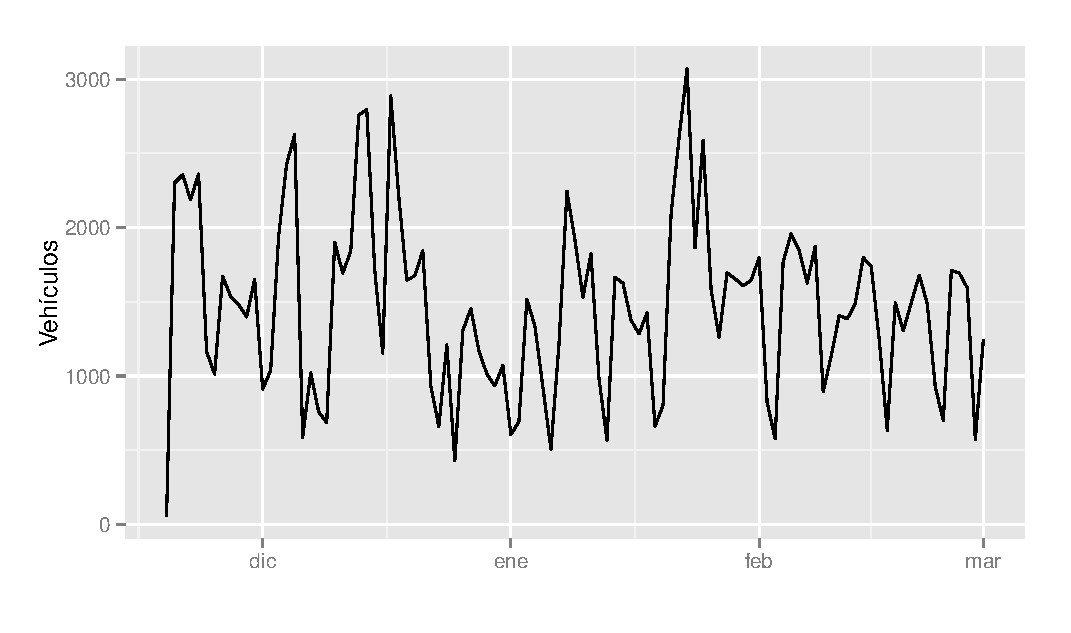
\epsfig{file=serieej.eps,width=14cm} 
\caption{Plot of the time series in the CSV file days\_1351591695721\_2012-11-19\_2013-03-01\_103\_55-3071\_.csv}
\label{fig:seriesEJ}
\end{figure*}


For example, the CSV file: \\
{\scriptsize {\tt days\_1351591695721\_2012-11-19\_2013-03-01\_103\_55-3071\_.csv}}  \\
corresponds to the time series in CSV format, covering the period from 11/19/2012 to 01/03/2013, at intervals of days, and whose data has been obtained in the node with id 1351591695721. 
In addition, this series is composed by 103 values, with the minimum at value 55 and the maximum at value 3071, and it does not include timestamp (TS).
The time series in this sample file is shown graphically in Figure \ref{fig:seriesEJ}.

Furthermore, due to the problem at hand and especially the type of hardware used, there are some times when the nodes do not detect any device. This might happend either because there is a period without passing vehicles, or because the monitoring node has stopped working ).
In such cases, the number of vehicles detected is zero.
That is why time series with missing values are offered. These time series are noted with the AN substring as part of the filename.
Missing values are marked with the NA value in the time series.

Finally, note that not only described time series have been offered, but also raw data has been left available in folder \emph{raw}.
Raw data, together with some functions developed using language R (included in the \emph{script} repository folder) might allow any researcher to generate new time series according to his needs (not restricted to those that have been generated and published).


%********************************************************************************
\section{Forecast accuracy measures}
\label{sec:medidasdeerror}



%********************************************************************************
\section{Time series prediction methods}



%********************************************************************************
\section{Obtained results}



%********************************************************************************
\section{Conclusions and future work}



%********************************************************************************
\section*{Acknowledgements}
This work has been supported in part by SIPESCA (Programa Operativo FEDER de Andaluc�a 2007-2013), TIN2011-28627-C04-02 and TIN2014-56494-C4-3-P (Spanish Ministry of Economy and Competitivity), SPIP2014-01437 (Direcci{\'o}n General de Tr{\'a}fico), PRY142/14 (Fundaci{\'o}n P{\'u}blica Andaluza Centro de Estudios Andaluces en la IX Convocatoria de Proyectos de Investigaci{\'o}n), and PYR-2014-17 GENIL project (CEI-BIOTIC Granada).


%********************************************************************************
\bibliographystyle{plain}
\bibliography{refs}

\end{document}
